\chapter{Specific Requirements}
This section is devoted to a specific description of every kind of requirement the
system has to deal with in order to achieve all the functionalities described.

\section{External interface Requirements}
\subsection{User Interfaces}
Figures below will present the hypothetical early phase user interfaces of the core functions of the system.

\vspace{0.5cm}
\begin{minipage}{.5\textwidth}
	\centering
	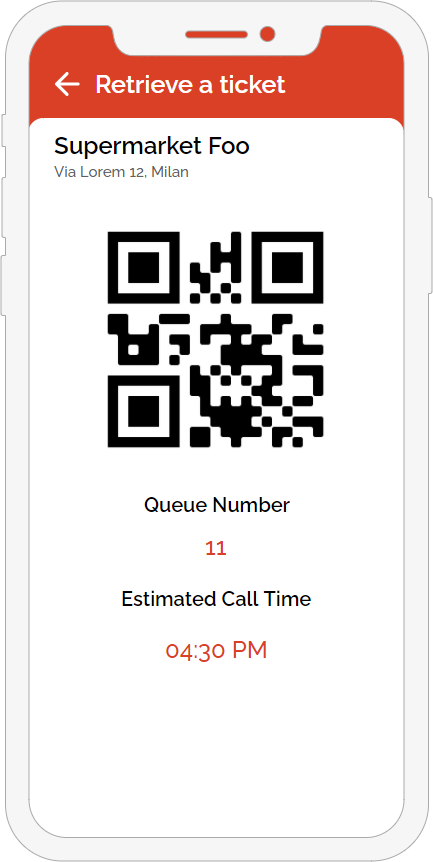
\includegraphics[width=0.9\textwidth]{ticket}
	\captionsetup{type=figure}
	\caption{Ticket page.}
\end{minipage}%
\begin{minipage}{.5\textwidth}
	\centering
	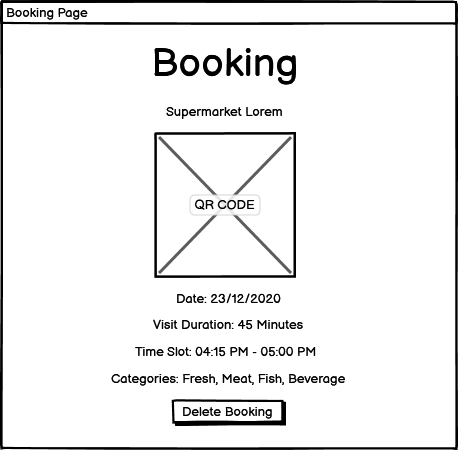
\includegraphics[width=0.9\textwidth]{booking}
	\captionsetup{type=figure}
	\caption{Booking page.}
\end{minipage}

\clearpage

\begin{minipage}{.5\textwidth}
	\centering
	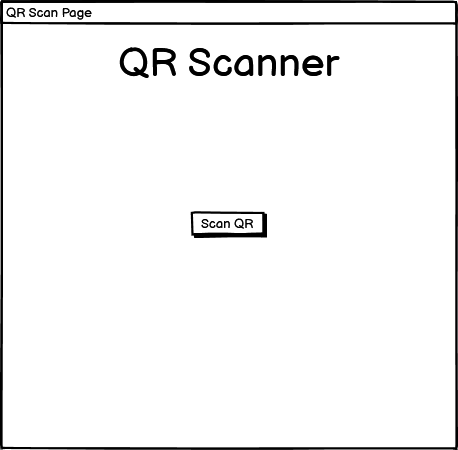
\includegraphics[width=0.9\textwidth]{scan}
	\captionsetup{type=figure}
	\caption{QR Scan page.}
\end{minipage}%
\begin{minipage}{.5\textwidth}
	\centering
	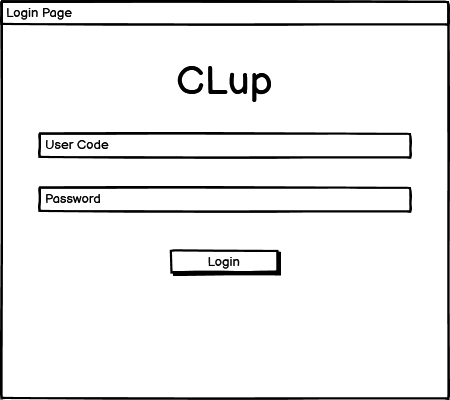
\includegraphics[width=0.9\textwidth]{login}
	\captionsetup{type=figure}
	\caption{Login Page.}
\end{minipage}

\bigskip\bigskip

\begin{minipage}{.5\textwidth}
	\centering
	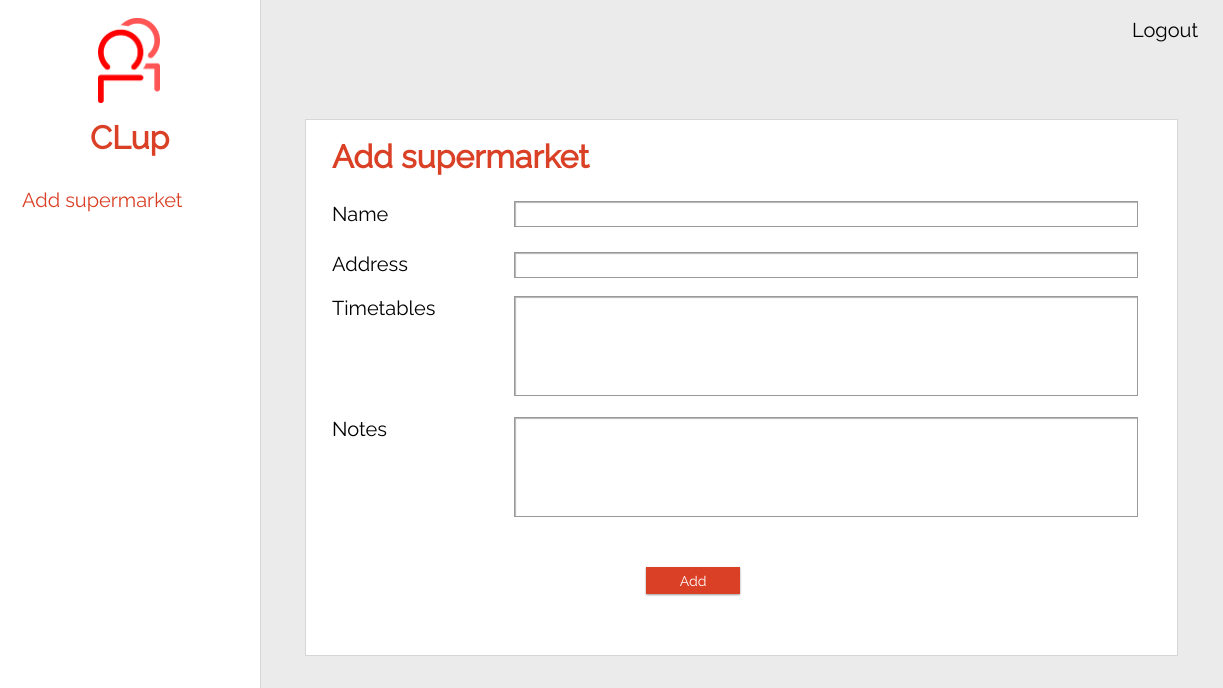
\includegraphics[width=0.9\textwidth]{new_store}
	\captionsetup{type=figure}
	\caption{New Store page.}
\end{minipage}%
\begin{minipage}{.5\textwidth}
	\centering
	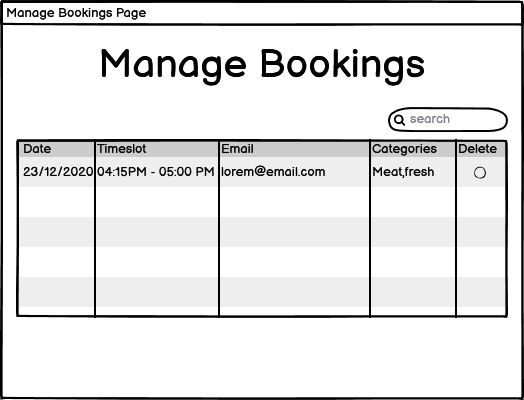
\includegraphics[width=0.9\textwidth]{manage_bookings}
	\captionsetup{type=figure}
	\caption{Manage Bookings page.}
\end{minipage}

\clearpage

\subsection{Hardware Interfaces}
In order to operate correctly, the system needs several devices which supermarkets shall acquire:
\begin{itemize}
	\item smartphones equipped with camera module for employees (one for the store entrance staff and one for each cash desk);
	\item a device with an attached display to show the store pass calls at the entrance;
	\item a tablet connected with a printer to setup the local Ticketing Kiosk.
\end{itemize}

For the normal usage, customers enjoy CLup using smartphones and their GPS module.
Store managers, store employees and CLup admins will access CLup services through web browser of their devices.

\subsection{Software Interfaces}
The system interfaces with a external map service for computing the distance between current place and store.

\subsection{Communication Interfaces}
All the communications from and to CLup are made via HTTPS.

\section{Functional Requirements}
In this section, it is given a complete description of the functional requirements of the system.

    \subsection{Requirements}
    \subsubsection{Customer}
        \begin{enumerate}[series=requirements, label=\textbf{R.\arabic*}]
            \item \itemtext{req:custQueue}{The system shall allow customers to line-up remotely in a store queue.}
            \item \itemtext{req:custTicket}{The system shall generate a new ticket when a customer enters a queue.}
            \item \itemtext{req:custTicketKiosk}{The system shall allow customers which do not have a smartphone to get a ticket in place.}
            \item \itemtext{req:custNum}{The system shall allow customers to view the number of people lined up in a queue.}
            \item \itemtext{req:custTime}{The system shall give customers an estimated waiting time.}
            \item \itemtext{req:custGps}{The system shall fetch the GPS position while the user has retrieved a store pass.}
            \item \itemtext{req:custLeave}{The system shall allow customers to leave a queue.}
            \item \itemtext{req:custFilter}{The system shall allow customers to filter stores by name.}
            \item \itemtext{req:custTtl}{The system shall notify customers when it's time to leave for the store.}
            \item \itemtext{req:custBook}{The system shall allow customers to book-a-visit to the store and send them the confirmation link and receipt via email.}
            \item \itemtext{req:custItems}{The system shall allow book-a-visit customers to specify the main categories of item they intend to buy.}
            \item \itemtext{req:custDelete}{The system shall allow customers to delete a store pass.}
            \item \itemtext{req:custNotifyDelete}{The system shall notify customers when a ticket or booked visit is deleted.}
            \item \itemtext{req:balanceBooking}{The system shall accept bookings based onto the already booked category items.}
        \end{enumerate}

    \subsubsection{Store manager}
    \begin{enumerate}[resume*=requirements]
        \item \itemtext{req:mngLogin}{The system shall allow a registered store manager to login by using their credentials.}
        \item \itemtext{req:mngViewStore}{The system shall allow store managers to view the current status of people inside the store.}
        \item \itemtext{req:mngViewQueue}{The system shall allow store managers to view the current status of people in the queue.}
         \item \itemtext{req:mngViewBook}{The system shall allow store managers to view the booked visits to the store.}
        \item \itemtext{req:mngCapStore}{The system shall allow store managers to set a maximum cap of people inside the store.}
        \item \itemtext{req:mngDeleteTickets}{The system shall allow store managers to delete tickets and booked visits.}
    \end{enumerate}

    \subsubsection{Store employee}
    \begin{enumerate}[resume*=requirements]
        \item \itemtext{req:stfLogin}{The system shall allow a registered store employee to login by using their credentials.}
        \item \itemtext{req:stfViewStore}{The system shall allow store employee to view the current status of people inside the store.}
        \item \itemtext{req:stfViewQueue}{The system shall allow store employee to view the current status of people in the queue.}
        \item \itemtext{req:stfQrCode}{The system shall allow store employee to scan QR codes.}
        \item \itemtext{req:stfValidatePass}{The system shall allow store employee to validate store passes.}
    \end{enumerate}

    \subsubsection{CLup admin}
    \begin{enumerate}[resume*=requirements]
        \item \itemtext{req:admRegister}{The system shall allow CLup admins to register new supermarkets.}
        \item \itemtext{req:admCredentials}{The system shall generate new manager and staff credentials for each supermarket registered.}
    \end{enumerate}

    \subsection{Goal mapping on requirements}

    \begin{description}


        \item \textbf{\printitem{goal:avoidQueue}}

        \begin{description}

        	\item \textbf{\printitem{goal:custHazardSit}}

			\printitem{req:custQueue}
			\printitem{req:custNum}
			\printitem{req:custTime}
			\printitem{req:custTtl}
			\printitem{req:custBook}
			\printitem{req:custItems}
			\printitem{req:balanceBooking}

			\printitem{dom:smartphone}
			\printitem{dom:categories}
			\printitem{dom:custEmail}
			\printitem{dom:oneToOneQr}
			\printitem{dom:timeArrival}


			\item \textbf{\printitem{goal:storeHazardSit}}

			\printitem{req:balanceBooking}
			\printitem{req:mngViewStore}
			\printitem{req:mngViewQueue}
			\printitem{req:mngViewBook}
			\printitem{req:mngCapStore}
			\printitem{req:mngDeleteTickets}
			\printitem{req:stfViewStore}
			\printitem{req:stfViewQueue}

			\printitem{dom:categories}
			\printitem{dom:oneToOneQr}
			\printitem{dom:internetStores}
			\printitem{dom:pecStores}
			\printitem{dom:employeeEntrance}
			\printitem{dom:timeArrival}
			\printitem{dom:capStores}


            \item \textbf{\printitem{goal:shortenTime}}

           	\printitem{req:custQueue}
           	\printitem{req:custNum}
           	\printitem{req:custTime}
           	\printitem{req:custTtl}
           	\printitem{req:custBook}
           	\printitem{req:stfQrCode}
           	\printitem{req:stfValidatePass}

           	\printitem{dom:smartphone}
           	\printitem{dom:workingGps}
           	\printitem{dom:gpsPrecision}
           	\printitem{dom:bringSmartphone}
           	\printitem{dom:employeeEntrance}
           	\printitem{dom:empSmartphone}
           	\printitem{dom:empCamera}
           	\printitem{dom:timeArrival}


            \item \textbf{\printitem{goal:arriveOnTime}}

           	\printitem{req:custQueue}
           	\printitem{req:custNum}
           	\printitem{req:custTime}
           	\printitem{req:custGps}
           	\printitem{req:custTtl}
           	\printitem{req:custBook}

           	\printitem{dom:smartphone}
           	\printitem{dom:workingGps}
           	\printitem{dom:gpsPrecision}
           	\printitem{dom:bringSmartphone}
           	\printitem{dom:timeArrival}
		\end{description}

        \item \textbf{\printitem{goal:otherTasks}}

       	\printitem{req:custQueue}
       	\printitem{req:custNum}
       	\printitem{req:custTime}
       	\printitem{req:custTtl}
       	\printitem{req:custBook}

       	\printitem{dom:smartphone}
       	\printitem{dom:workingGps}
       	\printitem{dom:gpsPrecision}
       	\printitem{dom:custEmail}
       	\printitem{dom:bringSmartphone}
       	\printitem{dom:timeArrival}


        \item \textbf{\printitem{goal:easyExp}}

       	\printitem{req:custTicket}
       	\printitem{req:custNum}
       	\printitem{req:custTime}
       	\printitem{req:custLeave}
       	\printitem{req:custFilter}
       	\printitem{req:custBook}
       	\printitem{req:custDelete}
       	\printitem{req:custNotifyDelete}
       	\printitem{req:stfQrCode}
       	\printitem{req:stfValidatePass}

       	\printitem{dom:smartphone}
       	\printitem{dom:workingGps}
       	\printitem{dom:uniqueName}
       	\printitem{dom:empSmartphone}
       	\printitem{dom:storeKiosk}


        \item \textbf{\printitem{goal:enjoyService}}

       	\printitem{req:custQueue}
       	\printitem{req:custTicketKiosk}
       	\printitem{req:custBook}

       	\printitem{dom:smartphone}
       	\printitem{dom:internetStores}
       	\printitem{dom:pecStores}
       	\printitem{dom:storeKiosk}


        \item \textbf{\printitem{goal:monitorAccess}}

		\printitem{req:balanceBooking}
       	\printitem{req:mngLogin}
       	\printitem{req:mngViewStore}
       	\printitem{req:mngViewQueue}
       	\printitem{req:mngViewBook}
       	\printitem{req:stfLogin}
       	\printitem{req:stfViewStore}
       	\printitem{req:stfViewQueue}
       	\printitem{req:stfQrCode}
       	\printitem{req:stfValidatePass}
       	\printitem{req:admRegister}
       	\printitem{req:admCredentials}

       	\printitem{dom:internetStores}
       	\printitem{dom:pecStores}
       	\printitem{dom:employeeEntrance}
       	\printitem{dom:capStores}


        \item \textbf{\printitem{goal:knowInAdvance}}

       	\printitem{req:mngViewStore}
       	\printitem{req:mngViewQueue}
       	\printitem{req:mngViewBook}
       	\printitem{req:stfViewStore}
       	\printitem{req:stfViewQueue}

       	\printitem{dom:smartphone}
       	\printitem{dom:categories}
       	\printitem{dom:internetStores}
       	\printitem{dom:pecStores}


        \item \textbf{\printitem{goal:limitNumber}}

		\printitem{req:balanceBooking}
       	\printitem{req:mngCapStore}
       	\printitem{req:mngDeleteTickets}
       	\printitem{req:stfQrCode}
       	\printitem{req:stfValidatePass}

       	\printitem{dom:smartphone}
       	\printitem{dom:categories}
       	\printitem{dom:internetStores}
       	\printitem{dom:pecStores}
       	\printitem{dom:empSmartphone}
       	\printitem{dom:empCamera}
       	\printitem{dom:timeArrival}
       	\printitem{dom:capStores}

    \end{description}


    \subsection{Traceability matrix}

    \begin{table}[H]
	    \centering
	    \resizebox{0.85\textwidth}{!} {
	    \begin{tabular}{@{}p{0.08\linewidth}cccccccccccccccccccccc@{}}
	         \toprule
	         \textbf{Item} &
	         \ref{req:custQueue} &
	         \ref{req:custTicket} &
	         \ref{req:custTicketKiosk} &
	         \ref{req:custNum} &
	         \ref{req:custTime} &
	         \ref{req:custGps} &
	         \ref{req:custLeave} &
	         \ref{req:custFilter} &
	         \ref{req:custTtl} &
	         \ref{req:custBook} &
	         \ref{req:custItems} &
	         \ref{req:custDelete} &
	         \ref{req:custNotifyDelete} &
	         \ref{req:balanceBooking}\\
	         \midrule

	         \textbf{\prettyref{uc:retrieveTicket}} & \cmark & \cmark & & \cmark & \cmark & \cmark & & \cmark & \cmark \\
	         \textbf{\prettyref{uc:bookVisit}} & \cmark & & & & & \cmark & & \cmark & \cmark & \cmark & \cmark & & & \cmark \\
	         \textbf{\prettyref{uc:deletePass}} & & & & & & & \cmark & \cmark & & & & \cmark & \cmark \\
	         \textbf{\prettyref{uc:webLogin}} & \\
	         \textbf{\prettyref{uc:registerStore}} & \\
	         \textbf{\prettyref{uc:monitorBookings}} & \\
             \textbf{\prettyref{uc:validatePass}} & \\
	         \midrule
	         \ref{goal:custHazardSit} & \cmark & & & \cmark & \cmark & & & & \cmark & \cmark & \cmark & & & \cmark \\
	         \ref{goal:storeHazardSit} & & & & & & & & & & & & & & \cmark \\
	         \ref{goal:shortenTime} & \cmark & & & \cmark & \cmark & & & & \cmark & \cmark \\
	         \ref{goal:arriveOnTime} & \cmark & & & \cmark & \cmark & \cmark & & & \cmark & \cmark \\
	         \ref{goal:otherTasks} & \cmark & & & \cmark & \cmark & & & & \cmark & \cmark &\\
	         \ref{goal:easyExp} & & \cmark & & \cmark & \cmark & & \cmark & \cmark & & \cmark & & \cmark & \cmark \\
	         \ref{goal:enjoyService} & \cmark & & \cmark & & & & & & & \cmark \\
	         \ref{goal:monitorAccess} & & & & & & & & & & & & & & \cmark \\
	         \ref{goal:knowInAdvance} & \\
	         \ref{goal:limitNumber} & & & & & & & & & & & & & & \cmark \\

	         \bottomrule
	     \end{tabular}}
     	\caption{\textit{Traceability matrix} for requirements R.1 to R.14.}
 	 \end{table}

	 \begin{table}[H]
		 \centering
	     \resizebox{0.85\textwidth}{!} {
	     \begin{tabular}{@{}p{0.08\linewidth}cccccc|ccccc|cc@{}}
	         \toprule
	         \textbf{Item} &
	         \ref{req:mngLogin} &
	         \ref{req:mngViewStore} &
	         \ref{req:mngViewQueue} &
	         \ref{req:mngViewBook} &
	         \ref{req:mngCapStore} &
	         \ref{req:mngDeleteTickets} &

	         \ref{req:stfLogin} &
	         \ref{req:stfViewStore} &
	         \ref{req:stfViewQueue} &
	         \ref{req:stfQrCode} &
	         \ref{req:stfValidatePass} &

	         \ref{req:admRegister} &
	         \ref{req:admCredentials}\\
	         \midrule

	         \textbf{\prettyref{uc:retrieveTicket}} & & & & & & & & & & &\\
	         \textbf{\prettyref{uc:bookVisit}} & & & & & & & & & & & & &\\
	         \textbf{\prettyref{uc:deletePass}} & & & & & & & & & & & & &\\
	         \textbf{\prettyref{uc:webLogin}} & \cmark & & & & & & \cmark & & \cmark & & & \cmark \\
	         \textbf{\prettyref{uc:registerStore}} & & & & & & & & & & & & \cmark & \cmark \\
	         \textbf{\prettyref{uc:monitorBookings}} & \cmark & & & \cmark & & \cmark & & & & & & &\\
             \textbf{\prettyref{uc:validatePass}} & & & & & & & \cmark & \cmark & \cmark & \cmark & \cmark & &\\
	         \midrule
	         \ref{goal:custHazardSit} & & & & & & & & & & & & &\\
	         \ref{goal:storeHazardSit} & & \cmark & \cmark & \cmark & \cmark & \cmark & & \cmark & \cmark & &\\
	         \ref{goal:shortenTime} & & & & & & & & & & \cmark & \cmark & &\\
	         \ref{goal:arriveOnTime} & & & & & & & & & & & & &\\
	         \ref{goal:otherTasks} & & & & & & & & & & & & &\\
	         \ref{goal:easyExp} & & & & & & & & & & \cmark & \cmark & &\\
	         \ref{goal:enjoyService} & & & & & & & & & & & &\\
	         \ref{goal:monitorAccess} & \cmark & \cmark & \cmark & \cmark & & & \cmark & \cmark & \cmark & \cmark & \cmark & \cmark & \cmark\\
	         \ref{goal:knowInAdvance} & & \cmark & \cmark & \cmark & & & & \cmark & & & \\
	         \ref{goal:limitNumber} & & & & & \cmark & \cmark & & & & \cmark & \cmark & & \\

	         \bottomrule
	     \end{tabular}}
     	 \caption{\textit{Traceability matrix} for requirements R.15 to R.27.}
    \end{table}

	\begin{table}[H]
    \centering
        \begin{tabular}{@{}p{0.08\linewidth}ccccccc@{}}
            \toprule
            \textbf{Item} &
            \textbf{\prettyref{uc:retrieveTicket}} &
            \textbf{\prettyref{uc:bookVisit}} &
            \textbf{\prettyref{uc:deletePass}} &
            \textbf{\prettyref{uc:webLogin}} &
            \textbf{\prettyref{uc:registerStore}} &
            \textbf{\prettyref{uc:monitorBookings}} &
            \textbf{\prettyref{uc:validatePass}}\\
            \midrule

            \textbf{\prettyref{sc:first}\textcolor{clupgrapefruit}{1}} & \cmark & & & & & & \cmark \\
            \textbf{\prettyref{sc:second}\textcolor{clupgrapefruit}{2}} & & \cmark \\
            \textbf{\prettyref{sc:third}\textcolor{clupgrapefruit}{3}} & & & \cmark \\
            \textbf{\prettyref{sc:fourth}\textcolor{clupgrapefruit}{4}} & & & & \cmark & \cmark \\
            \textbf{\prettyref{sc:fifth}\textcolor{clupgrapefruit}{5}} & & & & \cmark & & \cmark \\

            \bottomrule
        \end{tabular}
        \caption{\textit{Traceability matrix} for scenarios and use cases.}
    \end{table}

\clearpage

\section{Performance Requirements}
This section specifies numerical requirements placed on the software or on human interaction with the software as a whole.\newline
All the computation will take place on the servers of the system, therefore the mobile apps shall be lightweight and occupy little memory on the smartphones.
Since the majority of stores usually open only during daytime, the load in the night is expected to decrease considerably.
Regarding the scan process to let people enter or exit the store, at least 95\% of the passes scan shall be processed in less than 1 second: this is required in order to fulfil the goals of CLup.

\section{Design Constraints}

\subsection{Standards Compliance}
The system will store all the data submitted to it in a standardized form. In this way, it will be easier to catalog, retrieve, and run queries on the data.

CLup system shall use stateless protocols and standard operations to allow components to be managed and updated without affecting the system as a whole.\newline
It’s crucial to design modules properly so that ease of use, security and performance will remain the core factors of the system.

\subsection{Other Constraints}
Regulatory policies have to be considered for the interaction between CLup and customers. The application, in fact, will ask the position of the customer while retrieving a store pass and while checking the pass status. Further information will be provided in the section \ref{req:privacy}.

\section{Software System Attributes}

\subsection{Reliability}
In order to guarantee continuity, services are required to be fault tolerant. Errors handling and fault containment mechanisms to prevent error propagation and data loss are to be arranged.

\subsection{Availability}
It is essential to have the lowest downtime possible, specially for the plain queue function (see section \clupref{desc:prodFunc}).
The ticketing components shall guarantee 99.9\% (\textit{three-nines}) of availability, so that only 8.76 hours of downtime per year are allowed.
Meanwhile the book-a-visit components shall guarantee 99\% (\textit{two-nines}) of availability, so that 3.65 days of downtime per year are allowed.

\subsection{Security}
The system shall perform role based access control (RBAC): an authorization scheme that grants access rights based on the role of the use. In particular, such components shall grant user authentication and authorization:
\begin{itemize}
    \item \textbf{Authentication}: request and verify the identity of CLup admin, store managers and employees attempting to login using a usercode and password.
    \item \textbf{Authorization}: verify the permissions of the logged user to perform any requested action (e.g. adding or removing a store, creating a new item category, etc.) before performing it.
\end{itemize}

\subsection{Maintainability}
The system shall be characterized by scalable and reusable modules which will be easier to maintain and replace in case of failure. Ordinary maintenance, for bug fixes and improvements, will be scheduled during night time, when the user traffic is minimal.\newline
The core aspects of maintainability and modularity will be addressed in the design document.

\subsection{Portability}
The web platform for store manager, staff and admin will be accessible by any web browser.\newline
The mobile application for customers must be accessible by as many users as possible, hence it must be developed for the major mobile OSes. Since the mobile apps do not demand special functions, a non native approach can be adopted to fasten the development process.
The server side has no major requirements for portability.

\subsection{Usability}
The mobile app and the web platform of the system will be designed to be concise and user-friendly, with a graphical interface to help users identify the proper choice on the screen. It is expected that the 95\% of the users will be able to complete tasks without requiring assistance.

\section{Other Requirements}

\subsection{Privacy Requirements}\label{req:privacy}
The system shall ensure that the collection and transmission of personal data is handled in accordance with user’s expectation and regulations.\newline
In fact, to protect customers privacy, only the strictly necessary user data are requested to enjoy the app. Ensuring users privacy is protected positively influences user’s experience, acceptance and continuous use of the platform. For instance the system shall block unauthorized access to implicit information (e.g. location) and encrypt data transmission.

\subsection{Installation requirements}
The complete solution shall be installed in the specified environment (i.e. a store) within 4 working days.\newline
Smartphones to be supplied to store employees shall be configured and CLup shall be installed onto them.\newline
No specific installation requirements are necessary from the customer point of view. Indeed a customer may install the app right before starting to use it.
